

\documentclass[xcolor={dvipsnames}]{beamer}
\usepackage{amsmath}
% \usepackage{beamerthemesplit} // Activate for custom appearance
\usepackage{hyperref}
\usepackage{ragged2e}
\usepackage{amssymb}
\usepackage{verbatim}
\usepackage{lmodern}



\title{Natural Language Processing}
\author{Schwartz}
\date{\today}



\begin{document}

\frame{\titlepage}

\frame
{
 \frametitle{The Sophomore Slump}

{
\fontfamily{<familyname>}\selectfont
\begin{quote}
\tiny
\justify

...or sophomore jinx or sophomore jitters refers to an instance in which a second, or sophomore, effort fails to live up to the standards of the first effort. It is commonly used to refer to the apathy of students (second year of high school, college or university), the performance of athletes (second season of play), singers/bands (second album), television shows (second seasons) and films (sequels/prequels). In the United Kingdom, the ``sophomore slump" is more commonly referred to as ``second year blues", particularly when describing university students. In Australia, it is known as ``second year syndrome", and is particularly common when referring to professional athletes who have a mediocre second season following a stellar debut. The phenomenon of a ``sophomore slump" can be explained psychologically, where earlier success has a reducing effect on the subsequent effort, but it can also be explained statistically, as an effect of the regression towards the mean.

\end{quote}
}

\begin{columns}
\begin{column}{.011\textwidth}
\end{column}
\begin{column}{.6\textwidth}
{
\fontfamily{<familyname>}\selectfont
\begin{quote}
\tiny
\justify

The concept of ``regression'' comes from genetics and was popularized by Sir Francis Galton's late 19th century publication of ``Regression towards mediocrity in hereditary stature.'' Galton observed that extreme characteristics (e.g., height) in parents are not completely passed on to offspring, but rather the characteristics in the offspring ``regress'' towards a mediocre point. By measuring the heights of hundreds of people Galton was able to quantify this ``regression'' and in so doing invented linear regression analysis, thus laying the groundwork for much of modern statistical modeling. The term ``regression'' stuck.
\end{quote}
}
\end{column}
\begin{column}{.4\textwidth}
\vspace{.1in}
%\hspace*{-.39in}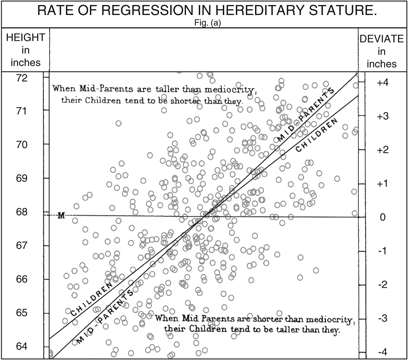
\includegraphics[width=1.55in]{galton.jpg} 

\end{column}
\end{columns}

% that the offspring of parents who lie at the tails of the distribution will tend to lie closer to the mean of the distribution. 

}

\frame
{
\normalsize
 \frametitle{Objectives}
\begin{itemize}
\item Terminology 
\item Least squares fit
\item Normal distribution theory  
\item Coefficient testing
\item Linear models and Multiple variables and Alternatives
\item Model fit and Model selection
\item Model diagnostics and Model evaluation
\end{itemize}

}

\end{document}

